\documentclass[a4paper,oneside,bibtotoc,smallheadings,pointlessnumbers,
halfparskip,DIV15]{scrartcl}
% kate: remove-trailing-space on; replace-trailing-space-save on; indent-width 2; indent-mode normal; space-indent on;
% tocleft,
\usepackage[pdftex]{graphicx}
\usepackage[ngerman]{babel}
\usepackage[utf8]{inputenc}
\usepackage{../../assets/uniinput}
\usepackage[T1]{fontenc}
\usepackage{amssymb,amsmath}
\usepackage{booktabs}
\usepackage{enumerate}
\usepackage{subfig}
% \usepackage{siunitx}
% \sisetup{
%   seperr         = true,
%   trapambigerr   = true,
%   openerr        = (,
%   closeerr       = ),
%   expproduct     = cdot,
%   padnumber      = both,
%   stickyper      = true,
%   per            = reciprocal,
%   trapambigfrac  = true,
%   repeatunits    = false,
%   openfrac       = (,
%   closefrac      = ),
%   prefixsymbolic = true,
%   prefixproduct  = cdot,
%   decimalsymbol  = comma,
%   tabnumalign    = left,
%   tabtextalign   = left
% }
\usepackage{color}
\definecolor{grey}{rgb}{.4,.4,.4}
\definecolor{darkgreen}{rgb}{0,.35,0}
\definecolor{ltgray}{gray}{0.95}
% \definecolor{darkblue}{rgb}{0,0,.6}
% \definecolor{darkred}{rgb}{.6,0,0}
% \definecolor{red}{rgb}{.98,0,0}
\usepackage{listings}
\lstdefinelanguage{Maxima}{
  keywords={addrow,addcol,zeromatrix,ident,augcoefmatrix,ratsubst,diff,ev,tex,%
    with_stdout,nouns,express,depends,load,submatrix,div,grad,curl,%
    rootscontract,solve,part,assume,sqrt,integrate,abs,inf,exp,float,log},
  sensitive=true,
  comment=[n][\itshape]{/*}{*/}
}
\lstdefinelanguage{C++}{
%   commentstyle=\itshape\color{darkgreen},
%   commentstyle=\color{darkgreen},
%   keywordstyle=\bfseries, %\color{darkblue},
%   stringstyle=\color{darkred},
%   basicstyle=\ttfamily\scriptsize,
  morekeywords={TH1F,TLorentzVector,TVector3,vector,TFile,TFitResultPtr,TF1,\
                TGraph,TH1,TObject,TCanvas,string,Double_t,TGraphErrors},
  basicstyle=\scriptsize,
  numbers=left,
  numberstyle=\tiny,%\color{gray},
  stepnumber=1,
  tabsize=4,
  showspaces=false,
  showstringspaces=false,
  breaklines=true,
  frame=lrtb,
  captionpos=b,
  extendedchars=true,
  inputencoding=utf8,
%   backgroundcolor=\color{ltgray}
}
% \usepackage{courier}
\lstset{language=Matlab,
%     keywords={break,case,catch,continue,else,elseif,end,for,function,global,if,otherwise,persistent,return,switch,try,while},
%     basicstyle=\ttfamily\small,%\scriptsize,
  basicstyle=\scriptsize,
  keywordstyle=\bfseries,
  commentstyle=\itshape\color{blue},
  stringstyle=\itshape,
  identifierstyle=\ttfamily,
  numbers=left,
  numberstyle=\tiny,
  stepnumber=1,
  tabsize=2,
  showspaces=false,
  showstringspaces=false,
  breaklines=true,
  frame=single,
  columns=fixed,
  captionpos=b,
  extendedchars=\true,
  inputencoding=utf8,
  backgroundcolor=\color{ltgray},
  postbreak = \raisebox{0ex}[0ex][0ex]{\ensuremath{\hookrightarrow}}
%   linewidth=0.9\textwidth
}
\usepackage[pdftex]{hyperref}
\hypersetup{
%   colorlinks  = true,
%   urlcolor    = darkblue,
  pdftitle    = {Protokoll zum CPII-Übungsblatt 3},
  pdfsubject  = {Protokoll Computational Physics}
  pdfauthor   = {robert.riemann@physik.hu-berlin.de,thomas.murach@physik.hu-berlin.de},
  pdfkeywords = {Computational Physics,CP,II,2010,Jacobi-Methode,Diagonalisierung,Eigenwerte, Eigenvektoren,eig,octave,matlab}
%   pdfcreator  = {pdftex},
%   pdfproducer = {pdftex}
}

\newcommand{\dd}[1]{\mathrm{d}#1\,} % declare dx operator, usage: \dd{x} for dx
\newcommand{\lref}[1]{Listing (\ref{lst:#1})} % refer to a listing, usage: \lref{label} for Listing (...)
\newcommand{\fref}[1]{Abb. (\ref{fig:#1})} % refer to a figure, usage: \lref{label} for Abb. (...)
\newcommand{\tref}[1]{Tab. (\ref{tab:#1})} % refer to a table, usage: \lref{label} for Tab. (...)
\newcommand{\eref}[1]{Gl. (\ref{eqn:#1})} % refer to a equation, usage: \lref{label} for Tab. (...)

\begin{document}
% % % % % % % % % % % % % % % % % % % % % % % %
\title{{\centering \rule{15cm}{0.001cm}\\
\Large{\textsc{Institut für Physik der
Humboldt-Universität zu Berlin}}}\\ \centering \rule{15cm}{0.001cm}\\
\vspace{15mm} \centering

\includegraphics[scale=0.9]{../../assets/siegel}\\
\vspace{18mm}
{\bf{\huge{Computational Physics II}}}\\
\vspace{12mm}
Übungsblatt 3\\
\vspace{15mm}
% Compton-Effekt\\
% \vspace{14mm} {\small{\textbf{Betreuer: M. zur Nedden}}}\\}
}
\author{Robert Riemann; Matr.Nr.: 521085\\
Thomas Murach; Matr.Nr.: 517771\vspace{18mm}}
% \vspace{8mm}
% \date{15. Juni 2008}
% % % % % % % % % % % % % % % % % % % % % % % %
% \onecolumn
\maketitle
% \twocolumn

\newpage
% \tableofcontents
% \listoffigures
% \listoftables
\section*{Aufgabe 3.1a}
Im ersten Teil der Aufgabe war zu untersuchen, wie sich die logistische
Abbildung $$M(x) = rx\cdot (1-x)$$ für $r$-Werte von 4, 3.9 und 3.832 verhält.
Im Speziellen wurde das invariante Maß $ϱ(x)$ untersucht, indem für 1000 zu
iterierende Punkte die erreichten $x$-Werte histogrammiert wurden. Der
Quelltext, der dies umsetzt, ist in \lref{logabb} dargestellt.

\lstinputlisting[firstline=1,firstnumber=1,label=lst:logabb,caption={logabb.m}]{
../logabb.m}

Die hierin aufgerufenen Funktionen sind in \lref{logmap} und \lref{logmapp}
dargestellt.

\lstinputlisting[firstline=1,firstnumber=1,label=lst:logmap,caption={logmap.m}]{
../logmap.m}

\lstinputlisting[firstline=1,firstnumber=1,label=lst:logmapp,caption={logmapp.m}
]{../logmapp.m}

Die Vorlagen für die Quelltexte stammen aus der Vorlesung. 

Die resultierenden Plots sind in \fref{logabb} dargestellt.
\begin{figure}[htb]
\centering
  \includegraphics[width=1\columnwidth,keepaspectratio]{../logabb.png}
  \caption{Output des Programms}
  \label{fig:logabb}
\end{figure}
% \section*{3.1b)}

Zu zeigen ist der Zusammenhang, der zwischen der logistischen Abbildung mit $r = 4$
\begin{equation}
 M_L(x_n) = 4x_n(1-x_n) = x_{n+1}
 \label{eqn:ml}
\end{equation}
und der Dreiecksabbildung
\begin{equation}
 \label{eqn:md}
 M_D(x_n) = \left(1-2\left|\frac{1}{2}-x\right|\right) = x_{n+1}
\end{equation}
besteht.

Nun substituieren wir $x_n$ in \eref{ml} mit:
\begin{equation}
 x_n = \sin^2\left(\frac{\pi}{2}\alpha_n\right)
\end{equation}
Hierbei wird darauf geachtet, dass die Substitution selbst auch eine Abbildung
von $[0, 1]$ nach $[0, 1]$ darstellt. Man erhält:
\begin{eqnarray}
 M_L(x_n) = x_{n+1} &=& 4x_n(1-x_n) \\
 \sin^2\left(\frac{\pi}{2}\alpha_{n+1}\right) &=& 4\sin^2\left(\frac{\pi}{2}\alpha_n\right)\underbrace{\left(1-\sin^2\left[\frac{\pi}{2}\alpha_n\right]\right)}_{\cos^2\left(\frac{\pi}{2}\alpha_n\right)} \\
 &=& 4\left[ \sin\left(\frac{\pi}{2}\alpha_n\right)\cos\left(\frac{\pi}{2}\alpha_n\right)\right]^2 = 4 \left[ \frac{1}{2} \sin\left( 2 \frac{\pi}{2} \alpha_n \right) \right]^2 = \sin^2\left(\frac{\pi}{2}2\alpha_n\right) \\
 \rightarrow \alpha_{n+1} &=& \pm 2 \alpha_n
\end{eqnarray}

Wie aus der Vorlesung bekannt ist, hat die logistische Abbildung ebenfalls eine
Stretching-Wirkung mit Faktor 2. Das Vorzeichen hängt hierbei von $x$ ab und ist
für Werte $\in [0; 0.5]$ positiv.

Darauf folgt die Equivalenz des invarianten Maßes der Dreiecksabbildung $ρ_D = 1$
und der logistischen Abbildung in Abhängigkeit von $alpha$ $ρ_L(α)$:
\begin{equation}
 ρ_D = ρ_L(α) = 1 
\end{equation}
Es gilt weiterhin:
\begin{eqnarray}
 ρ_L(α)\dd{α} &=& ρ_L(x)\dd{x} \\
  \rightarrow ρ_L(x) &=& \underbrace{ρ_L(α)}_{=1} \frac{\dd{\alpha}}{\dd{x}} \\
 \frac{\dd{x}}{\dd{α}} &=&  π \sin\left(\frac{\pi}{2}\alpha\right)\cos\left(\frac{\pi}{2}\alpha\right) = π\sqrt{x(1-x)} \\
 \rightarrow ρ_L(x) &=& \frac{1}{\pi\sqrt{x(1-x)}}
\end{eqnarray}

Der Vergleich zwischen experimentellem und theoretischem Ergebnis ist in \fref{1b}
veranschaulicht. Die rote Line beschreibt den auf die experimentellen Daten
renormierten theroretischen Verlauf $ρ_L(x)$.
\begin{figure}[htb]
\centering
  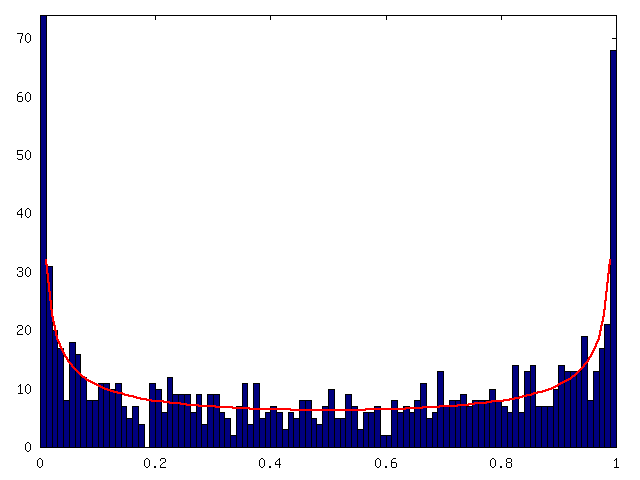
\includegraphics[width=1\columnwidth,keepaspectratio]{../logabb_r4.png}
  \caption{Vergleich zwischen Experiment und Theorie von $ρ_L(x)$}
  \label{fig:1b}
\end{figure}






\section*{Aufgabe 8.2}
In dieser Aufgabe sollte die Dichte in Abhängigkeit der Dichte für verschieden Gittergrößen
geplottet werden. Der Code dafür ist bereits in \lref{bond_perk} dargestellt. Die
resultierenden Kurven sind in \fref{dichte} dargestellt.

\begin{figure}[htb]
  \centering
  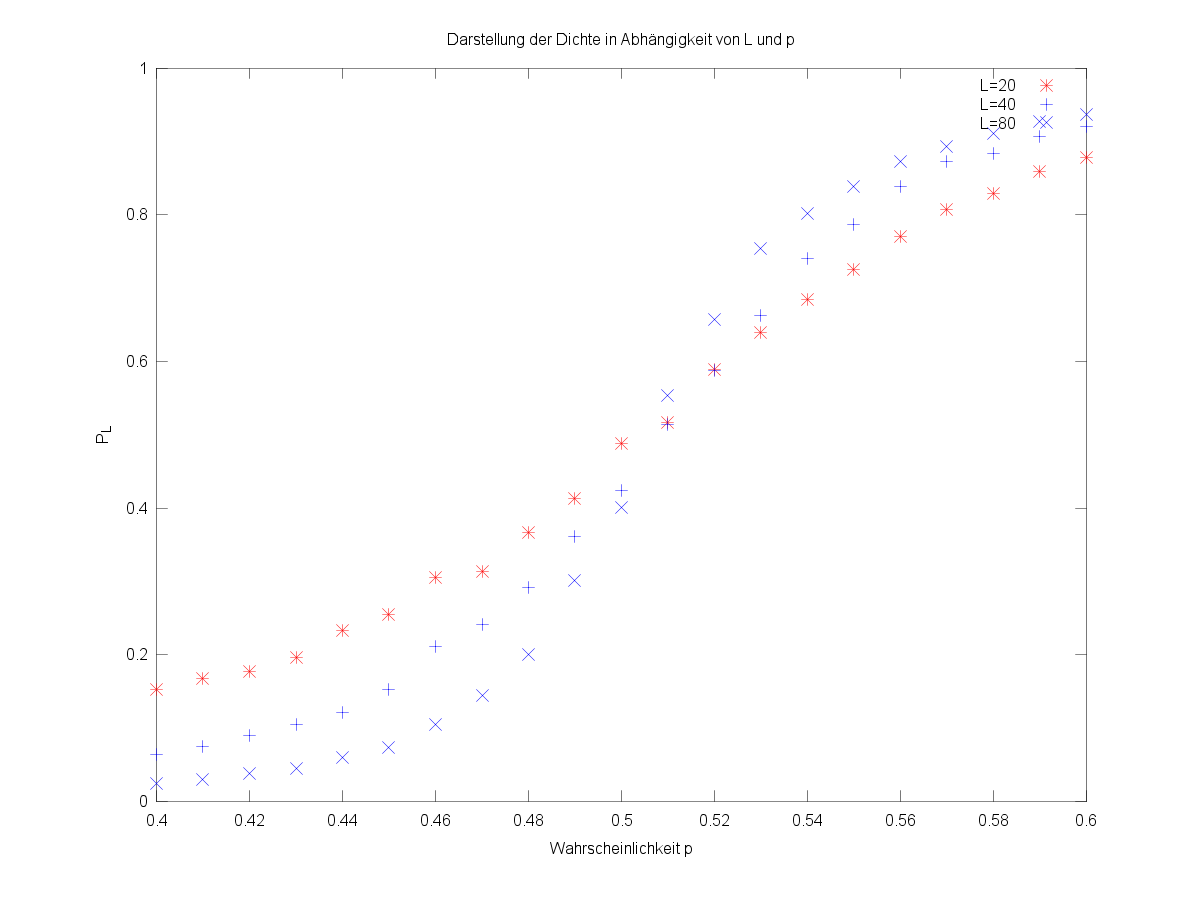
\includegraphics[width=0.8\columnwidth,keepaspectratio]{../tmp/zweitens.png}
  \caption{Dichte in Abhängigkeit von der Wahrscheinlichkeit und für verschiedene Gittergrößen}
  \label{fig:dichte}
\end{figure}

Man erwartet für $p<0.5$, dass die Dichte für sehr große Gitter gegen null geht 
und für größere Wahrscheinlichkeiten gegen 1. Dies kann hier nicht exakt erreicht werden,
da nur endliche Gitter verwendet wurden, aber die entsprechende Tendenz ist erkennbar.
Aufgrund der relativ langwierigen Programmausführung wurde sich auf drei Messwerte beschränkt.
% \input{auswertung}
% \input{ergebnis}
% \input{quellen}
% \input{anhang}

% \section{Beispiele}
% blabla
%
% Weitere Information sind der Versuchsbeschreibung im \cite{script} zu entnehmen.
%
% \lstinputlisting[firstline=2,firstnumber=1,label=lst:aufruf,caption={aufruf.m - Matlab Batchdatei}]{aufruf.m}
%
% \begin{eqnarray}
% 	g &=& \SI{9.8157(11)}{\metre\per\second\squared} \\
%         \left[ g \right] &=& \si{\metre\per\Square\second} % großschreibung!
% 	\label{eqn:asdf}
% \end{eqnarray}
%
% Dann kann man auf \eref{asdf} verweisen.


% \begin{figure}[htb]
% 	\centering
% 	\includegraphics[width=1\columnwidth,keepaspectratio]{Winkelabhaengigkeit2}
% 	\caption{Periodendauer in Abhängigkeit der Maximalauslenkung}
% 	\label{fig:Winkelabhaengigkeit}
% \end{figure}

% \begin{table}[htbp]
% \centering
% \setlength{\tabcolsep}{14pt}
% \begin{tabular*}{\columnwidth}{%
% S[tabformat=2.1]%
% S[tabformat=2.2]%
% S[tabformat=1.2]}
% \toprule
% {$R$ in \si{\ohm}} &
% {$U$ in \si{\volt}} &
% {$\frac{U}{U_{R=0}}$}\\
% \midrule
% \multicolumn{3}{c}{\textit{Eingangswiderstand $R_E$}}\\
% \midrule
% 0 & 16 & 1 \\
% 4.7e3 & 8 & 0.5 \\
% \midrule
% \multicolumn{3}{c}{\textit{Ausgangswiderstand $R_A$}}\\
% \midrule
% 0 & 1.8 & 1 \\
% 12 & 0.52 & 0.29 \\
% 27 & 1.2 & 0.67 \\
% 18 & 0.8 & 0.44 \\
% \bottomrule
% \end{tabular*}
% \label{tab:221messungexp_widerstaende}
% \caption{experimentelle Messung der Ein- und Ausgangswiderstände}
% \end{table}


% \newpage

% \onecolumn
% \appendix
% \begin{figure}
% 	\centering
% 	\includegraphics[width=0.98\textwidth,keepaspectratio]{Messprotokoll}
% 	\caption{Messprotokoll}
% 	\label{fig:protokoll}
% \end{figure}
%\colorbox{yellow}{} Farben verwenden
\end{document}
